\chapter{Synchronization} % Titlul capotilului
\label{Capitolul5}


As described in chapter \ref{Capitolul2}, the applications that use our library are take care of updating the monitored objects with the current operational values while in a separate thread the {\tt monsvc} library samples these objects and sends them to an IS server. This concurrent access pattern creates problems which include issues regarding visibility of updates of one thread in another one and accessing data structures in inconsistent state. Therefore, we need to synchronize the access to the monitored objects between application and library threads.

\section*{Smart pointers}

We use smart pointers in order to implement the synchronization between the application and the library while requiring only minimal and incremental changes to the existing codebase. For every object registered with the library we return a smart pointer that is used by both library and application as a proxy for accessing the registered object. 

The smart pointers offer a simple interface to the application developer. They have two functions called lock and unlock which ensure exclusive access to the underlying object. Moreover, we use an interesting C++ feature \citep{andrei2001modern} that allows us to overload the dereference operator to lock the smart pointer just before any method call or field access and unlock it afterwards.

Due to the nice syntactical similarities between smart pointers and raw pointers we can easily port the code to use the former. It usually requires just changing the type of the declaration of the pointer. For example, the following function can be ported just by changing the type of the parameter:
\input{Code/dow1}
to obtain the following form:
\input{Code/dow2}
As explained above, the smart pointer takes care of the synchronization with the library on every function call and field access.

There is an exception to the previous case in which the pointer should be passed to a legacy function which we cannot change. For example:
\input{Code/dow3}
in which case we replace it with:
\input{Code/dow4}
Note that in this case even the change was very small, there is a trade-off between lock granularity and the amount of code that needs to be changed. For example, if we had ten calls to legacy functions and each of them was fast, we could as well lock around the \verb+do_work+ to save the refactoring work.

\section*{Synchronization strategies}
In the previous section we referred to locking and unlocking the smart pointer without giving details about how this is implemented. In this section we will present different implementations among which the application developer can choose when registering an object.

\subsection*{No synchronization}

The information that is stored in the IS server is represented as objects with the base class ISInfo. Some of these objects are generated from XML description. We implemented a script which can generate a thread-safe version of the object which uses atomic integers for the fields. 

In cases where this level of thread-safety is sufficient, a developer can avoid the overhead of locking by using a smart-pointer that provides no synchronization.

\subsection*{Mutex}

The simplest synchronization policy is to acquire mutex when accessing the object. The disadvantage of this strategy is that the library has to lock the object while it sent over the network to the IS server. This is because the publishing to the IS server uses a legacy function similar with the example we have given before.

\subsection*{Copy before publish}

When using this synchronization strategy, the library makes local copy of the object before publishing it to the IS server. The advantage of this technique is that we avoid holding a lock while sending the object over the network. The disadvantage is that we consume more time and memory to make a copy of the object which may not be acceptable for large histograms.

This strategy is the opposite of copy-on-write but we prefer it since in our case the object is written more often than is read.

\subsection*{Asynchronous updates}

An important observation which we can leverage is that in our use cases, the application that updates an object with the current operational values does not need to wait for the update to be applied. All we are interested in is serial consistency of the operations on that object. 

With the asynchronous updates strategy, we still use a mutex to ensure exclusive access to the underlying object. The only difference is that when the application tries to update a locked object it just enqueues the update to be applied at a later time. Our updates usually increment a counter or a histogram bin, hence they can be represented very compactly making this strategy lightweight in terms of space usage. It also avoid blocking the main application threads while sending the monitored objects over the network.

The interface of the smart pointer that implements this strategy leverages the C++11 variable argument templates to provides asynchronous updates to any type of monitored object. The declaration of the method responsible with asynchronous updates is the following:
\input{Code/async_ptr}

This method takes a pointer to a member function and its arguments and calls it asynchronously. It requires to change the method calls of the from \verb+h->observe(42)+ to use the following form: \verb+h.async(Histo::observe, 42);+.

Another positive point of this implementation is that we can rewrite only some of the method calls to be asynchronous, so there is again a trade-off between the amount of code to be modified and performance.

\subsubsection*{Intuition}

The figure \ref{fig:sync_ptr} represents the operation of the locking strategy while the figure \ref{fig:async_ptr} corresponds to the asynchronous updates strategy. One can see that in the second case, the application thread is not disturbed by the monitoring thread which is publishing the object that it is trying to update.
\begin{figure}[ht!]
\centering
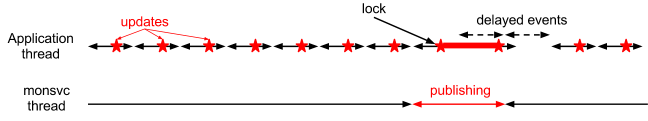
\includegraphics[scale=0.6]{Images/async_before.png}
\caption{Locking strategy}
\label{fig:sync_ptr}
\end{figure}

\begin{figure}[ht!]
\centering
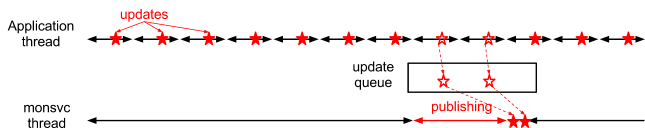
\includegraphics[scale=0.6]{Images/async_after.png}
\caption{Asynchronous updates strategy}
\label{fig:async_ptr}
\end{figure}

\subsubsection*{Implementation}

In this section we will present the implementation of the main operations of the smart pointer. The dereference operator is implemented on top of these operations. The smart pointer class has the following fields:
\begin{itemize}
\item {\tt update\_queue} the queue of updates that need to be executed asynchronously.
\item {\tt qlock} a mutex used to protect the {\tt update\_queue}.
\item {\tt obj\_lock} a mutex used to protect the object pointed by the smart pointer.
\end{itemize}
And the pseudocode is given below:
\input{Code/async}
Note that the {\tt async} method does not block when trying to acquire {\tt obj\_lock} since it uses the non-blocking {\tt try\_lock} method. 

Every thread that acquires the {\tt obj\_lock} mutex executes all updates that were added to the {\tt update\_queue} before accessing the underlying object of the smart pointer. This way we ensure that after the exclusive access to the object is given to the application, the object is in a serially consistent state. As an optimization, we also execute all updates before releasing the {\tt obj\_lock}.

\subsubsection*{Custom mechanisms}

We also provide a smart pointer that uses callbacks to allow user to implement its own synchronization mechanisms such as, for example, per-cpu counters that are added up only before being read.
